% -*-coding: utf-8 -*-

Připomeňme, že nás nyní \emph{nezajímá} rychlost konvergence algoritmů, nebo přesněji veličina $\frac{\text{doba konvergence}}{\text{počet vyčíslení účelové funkce}}$. Ta je velmi závislá na úloze, nastavení parametrů algoritmu a~paralelizace ji -- až na zmíněný efekt superlineárního urychlení -- příliš neovlivní. \emph{Nyní nás zajímá doba výpočtu jednoho kroku algoritmu (jedné generace) a zkrácení této doby při použití GPU}.

\section{Příprava testování}
\subsection{Hardware}

Hardwarová sestava pro testy byla následující:

\begin{table}[h]
    \begin{center}
    \begin{tabular}{lcc}
      \toprule
      & CPU & GPU \\
      \midrule
      Název & AMD Phenom$^\mathrm{TM}$ II X4 945 & NVIDIA GeForce GTX 460 \\
      Výpočetní jednotky & 4 (využita 1) & 336 (7 SM $\times$ 48 CUDA-jader) \\
      Frekvence & 800 MHz & 675 MHz \\
      Výpočetní schopnost & --- & 2.1 \\
      Cache & 2 MB L2 & --- \\
      RAM/DRAM & 4 GB & 768 MB GDDR3 \\
      FSB & ? & 1800 MHz \\
      \bottomrule
    \end{tabular}
    \caption{Testovací sestava}
    \end{center}
\end{table}

Je nutné podotknout, že ani CPU, ani GPU zdaleka nejsou na špičce současných produktových řad. Při paralelizaci na dnešních nejvýkonnějších CPU (Intel Core i7 -- 4 jádra, 8 vláken, 3GHz) bychom mohli dosáhnout proti testovanému CPU teoretického urychlení cca $30\times$. Urychlení současné nejvýkonnější GPU (Nvidia GTX690 -- 3072 jader, 915Mhz, dvojnásobná rychlost zpracování instrukcí) oproti testované by se mohlo pohybovat kolem $25\times$. Technologický trend by tedy naše výsledky neměl výrazně vychýlit ve prospěch CPU.

\subsection{Testované algoritmy a použité účelové funkce}
Testovali jsem algoritmy náhodná střelba (RS), genetická optimalizace (GO), a simulované žíhání (SA). Jako účelové funkce jsem zvolili sférickou De Jongovu funkci č. 1 a problém \emph{sudoku}. De Jongova funkce č. 1 vypadá následovně:
\[
f_{DJ} = \sum_1^n x_i^2,
\]
kde $x_i$ je $i$-tá složka kandidáta. Počet dimenzí ($n$) byl nastaven na 5. Jednalo se tedy o~jednoduchý problém s nízkou dimenzí, kde by měla vyniknout kvalita paralelizace zbylé logiky algoritmu.

Problém \emph{sudoku} má simulovat hledání přípustného řešení za pomocí penalizační funkce. Úloha má 81 dimenzí, povolené hodnoty jsou celá čísla z $[1,9]$. Velikost penalizace odpovídá počtu konfliktů v řádcích, sloupcích a ve čtvercích. Úloha byla zvolena jako příklad většího, algoritmicky náročnějšího, avšak plně paralelizovatelného problému.

\subsection{Parametry algoritmů}

Uživatelské parametry u algoritmů byly zvoleny následovně:
\begin{itemize}
  \item RS: Nemá parametry.
  \item GO: Pravděpodobnost křížení: 50\% , pravděpodobnost mutace: 90\%, rozptyl mutace $\sigma^2 = 1$. Na rychlost výpočtu má vliv pouze pravděpodobnost křížení a mutace, neboť ta určuje, kolik dat se bude muset zpracovat.
  \item SA: Počáteční teplota: $10^6$, rozptyl mutace $\sigma^2 = 50$. Žádný z těchto parametrů však příliš neovlivňuje rychlost výpočtu.
\end{itemize}

U algoritmů jsme měřili, jak dlouho trvá spočítat 100 generací\footnote{Než algoritmus zkonverguje na reálném problému, trvá to běžně tisíce generací}. Na GPU byl spuštěn pro 20 různých konfigurací velikosti populace (32, 64, 128, 256, 512) a počtu paralelních populací (1, 10, 100, 1000). Na CPU jsme testovali jen 5 konfigurací se stejnými velikostmi populace, avšak pouze s jednou \bq paralelní\eq~ populací. U GO byla velikost potomstva nastavena vždy na dvojnásobek velikosti populace. V každé konfiguraci byl algoritmu spuštěn 50krát. Každý algoritmus byl tedy spuštěn pro každou účelovou funkci 1000krát na GPU a 250krát na CPU.

\subsection{Měření času}

K měření času jsme použili funkci \texttt{clock\_gettime} používající časomíru \texttt{CLOCK\_PROCESS\_} \texttt{CPUTIME\_ID}. Ta dává stabilní výsledky spotřebovaného času vlákna s přesností na nanosekundy. Při měření času na počítači se díky procesům v operačním systému (multitasking apod.) vyskytne několik hodnot ležících mimo hlavní shluk (outliers). Proto jako výsledný čas uvádíme \emph{median z oněch 50ti měření}. Do standardních odchylek jsou outliery započítány.

Měření bylo celkem stabilní, při absenci outlierů klesala směrodatná odchylka na GPU času pod 1\% naměřené hodnoty, na CPU pak pod 3\%.

\section{Výsledky}\label{vysledky}

Vzhledem k tomu, že se jedná $20\times 12$ konfigurací, kompletní tabulky lze nalézt v sekci \ref{app SP}, \ref{app SU}. Zde uvedeme jen nejlepší a nejhorší výsledné zrychlení pro každý algoritmus a~účelovou funkci. Uvedené časy jsou pro 100 generací. Připomeňme, že se jedná o \emph{medianové} časy. Výsledky pro De Jongovu sférickou funkci:

\begin{table}[h]
    \begin{center}
    \begin{tabular}{lccccc}
      \toprule
      algoritmus &  & zrychlení & konfigurace & čas GPU (ms) & čas CPU (ms) \\
      & & & (\# p. na GPU) & /1 populace & /1 populace \\
      \midrule
      \multirow{2}{*}{RS} & nejlepší & 90,5 & 256 (1000) & 0,12 & 10,86 \\
                        & nejhorší & 1,1 & 64 (1) & 2,49 & 2,74\\
      \multirow{2}{*}{GO} & nejlepší & 127,1 & 256 (1000) & 0,73 & 92,77\\
                        & nejhorší & 2 & 32 (1) & 5,76 & 11,3\\
      \multirow{2}{*}{SA} & nejlepší & 151,4 & 256 (1000) & 0,27 & 40,26 \\
                        & nejhorší & 1,3 & 32 (1) & 3,97 & 5,1\\
      \bottomrule
    \end{tabular}
    \caption{Extrémní výsledky pro De Jongovu sférickou funkci}
    \end{center}
\end{table}

Výsledky pro problém \emph{sudoku}:

\begin{table}[h]
    \begin{center}
    \begin{tabular}{lccccc}
      \toprule
      algoritmus &  & zrychlení & konfigurace & čas GPU (ms) & čas CPU (ms) \\
      & & & & /1 populace & /1 populace \\
      \midrule
      \multirow{2}{*}{RS} & nejlepší & 533,4 & 256 (1000) & 1,27 & 677,36\\
                        & nejhorší & 6,84 & 32 (1) & 12,4 & 84,77\\
      \multirow{2}{*}{GO} & nejlepší & 425,1 & 128 (1000) & 2,48 & 1055,6\\
                         & nejhorší & 6,62 & 32 (1) & 39,68 & 262,51 \\
      \multirow{2}{*}{SA} & nejlepší & 566 & 256 (1000) & 1,95 & 1102,1\\
                        & nejhorší & 4,96 & 32 (1) & 27,83 & 138,03\\
                       
      \bottomrule
    \end{tabular}
    \caption{Extrémní výsledky pro sudoku}
    \end{center}
\end{table}

Z hodnocení RS u De Jongovy funkce byl vyřazen první sloupec (32 jedinců v populaci), neboť na CPU byl algoritmus z nějakého důvodu pomalejší, což mohlo být způsobeno špatným využitím cache kvůli nevhodným střídám v algoritmu -- dále viz \ref{app SP}. Stejné chování nastává i na GPU pro malé populace, viz \ref{SP graphs}.

Dobrým výsledkem je, že u obou funkcí neběží algoritmy na GPU pomaleji než na CPU. Je to dáno tím, že i když je nutná jistá komunikace v populaci, mnoho komponent algoritmů je čistě paralelní. U De Jongovy funkce dosahujeme stabilního maximálního urychlení kolem 100 i přes, což je velmi slibné pro statistické testování chování různých OA, kde se většinou používá podobně výpočetně jednoduchá účelová funkce.

Všimněme si, že pro problém \emph{sudoku} dosahuje maximální zrychlení větších hodnot, než je počet CUDA jader na GPU (336), která mají navíc nižší frekvenci než CPU. Je to dáno jednak tím, že výpočet účelové funkce je čistě vektorový, takže paralelizace má největší možný efekt a dále tím, že maximální propustnost (a frekvence) paměti na GPU je mnohem větší než na CPU. Pokud je přístupů do paměti hodně a jsou ideálně uspořádané, může se vyšší takt GPU pamětí výrazně projevit. Že se nejedná o omyl dosvědčují i nehorší hodnoty urychlení, které jsou zhruba 4krát větší, než u De Jongovy funkce, tedy ve stejném poměru, jako nejlepší výsledky.

\begin{figure}[h!]
\begin{center}
  \includegraphics[width=\textwidth]{img/graphsSP}
  \caption{Přehledové grafy pro De Jongovu funkci}\label{SP graphs}
  \end{center}
\end{figure}
\clearpage

\begin{figure}[h!]
\begin{center}
  \includegraphics[width=\textwidth]{img/graphsSU}
  \caption{Přehledové grafy pro sudoku}\label{SU graphs}
  \end{center}
\end{figure}
\clearpage

Z přehledových grafů \ref{SP graphs}, \ref{SU graphs} je dobře vidět typické chování GPU. Vzhledem k tomu, že paralelizujeme většinu algoritmu způsobem populace na blok, zvýšení počtu populací nás z počátku nic nestojí, protože GPU má dostatek výpočetních zdrojů. Stejné je to při malé velikosti populace. Při větším počtu populací a jejich větších velikostech se karta začíná sytit. To je v grafech vidět na tam, kde závislost v obou osách přechází v lineární -- když tedy zdvojnásobíme (zdesetinásobíme) zadání, zdvojnásobí (zdesetinásobí) se čas výpočtu. 

Maximálního zrychlení většinou není dosaženo při největší velikosti populace (512), ale na poloviční, či čtvrtinové. GPU se totiž snaží využít veškeré prostředky, a když jsou bloky malé, umístí jich na jeden SM několik, čímž zlepší překrývání paměťových latencí. Pokud jsou bloky příliš velké, vejde se jich na SM méně s větším \bq zbytkem\eq , čímž se zhorší využití prostředků.

\section{Shrnutí}

Provedené testy prokázaly, že se model chová dobře pro několik celkem odlišných zástupců široké množiny OA. Pro jednoduché účelové funkce můžeme očekávat, že u ostatních algoritmů se při větším počtu paralelních populací ($>100$) zrychlení bude pohybovat na podobné hladině, tedy kolem hodnoty 100. Klíčem ke stabilně dobrému urychlení je optimální vytížení GPU pomocí většího počtu paralelních populací a případně úprava velikosti populace.

